\documentclass{article}

\usepackage[margin=1.4in]{geometry}
\usepackage[dvipsnames]{xcolor}
\usepackage{graphicx}
\graphicspath{ {./images/} }

\title{Transaction management in DBMS}
\author{Krishna Agrawal, 19111031}
\date{\today}

\begin{document}
\maketitle

\section*{Abstract}

Evolution in database systems applications are increasing day by day, 
accompanied by the emergence of many of the problems that are looking for a 
solution. Transactions are important primitives to provide reliability and controlled access to shared databases. The concepts of transaction management involving simple read,write transactions, ACID properties and enforcing serializability have already been discussed in this paper.


\section*{Introduction}

One of the major uses of DBMS is to protect the user’s data from system failures. It is done by ensuring that all the data is restored to a consistent state when the computer is restarted after a crash. The transaction is any one execution of the user program in a DBMS. Executing the same program multiple times will generate multiple transactions.

A transaction is a basic, atomic unit of consistent and reliable computing, composed of a sequence of atomic operation executions. 

The main problem that can happen during a transaction is that the transaction can fail before finishing all the operations in the set. This can happen due to power failure, system crash etc. This is a serious problem that can leave database in an inconsistent state. To solve this problem, we use commit and roll-back operations. Even though these operations can help us avoiding several issues that may arise during transaction but they are not sufficient when two transactions are running concurrently. To handle those problems we need to understand database ACID properties. 

Concurrency control is one of the techniques to be addressed by this 
paper, it is responsible for concurrent transaction, and permits users to access database in a safe state. 

\section*{Transaction management}
Transaction Management deals with the problems of always keeping the database in consistent state even when concurrent accesses and failures occur. A transaction is a collection of actions that make consistent transformations of system states while preserving system consistency. The consistency and reliability aspects of transactions are due to four following properties called ACID (Atomicity, Consistency, Isolation, and Durability). Atomicity ensures complete transaction execution, consistency in transaction correctness, isolation ensures transaction independence in parallel executions and durability refers to transaction persistence in database. 

\begin{figure}[h]
 \centering
 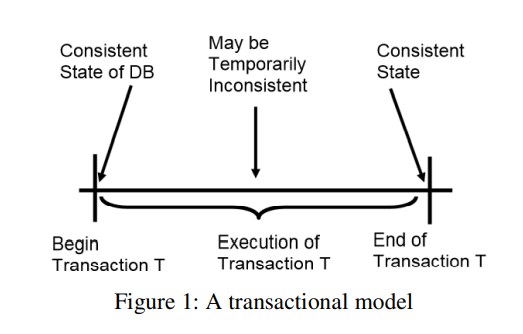
\includegraphics{model}
\end{figure}


Therefore, to ensure integrity of the data, we require that the database system maintain the ACID properties of the transactions.

\section*{Operations of Transaction}

Following are the main operations of transaction:

\begin{enumerate}


\item \textbf{Read(X)}: Read operation is used to read the value of X from the database and stores it in a buffer in main memory.

\item \textbf{Write(X)}: Write operation is used to write the value back to the database from the buffer.

Let's take an example to debit transaction from an account which consists of following operations:

1.  R(X); 
 
2.  X = X - 500;  

3.  W(X);  

Let's assume the value of X before starting of the transaction is 4000.
\begin{itemize}

\item The first operation reads X's value from database and stores it in a buffer.
\item The second operation will decrease the value of X by 500. So buffer will contain 3500.
\item The third operation will write the buffer's value to the database. So X's final value will be 3500.
\end{itemize}

But it may be possible that because of the failure of hardware, software or power, etc. that transaction may fail before finished all the operations in the set.

For example: If in the above transaction, the debit transaction fails after executing operation 2 then X's value will remain 4000 in the database which is not acceptable by the bank.

To solve this problem, we have two important operations:

\item \textbf{Commit:}  If all the operations in a transaction are completed successfully then commit those changes to the database permanently. 

\item \textbf{Rollback:}  If any of the operation fails then rollback all the changes done by previous
operations. 

\end{enumerate}

Even though these operations can help us avoiding several issues that may arise during
transaction but they are not sufficient when two transactions are running concurrently. To
handle those problems we need to understand database ACID properties.



\section*{Properties of Transaction}

A Transaction has four properties that lead to the consistency and reliability of a data base. These are Atomicity, Consistency, Isolation, and Durability which are combinedly named as ACID properties.
\begin{enumerate}


\item \textbf{Atomicity:}
This refers to the fact that a transaction is treated as a unit of operation. Consequently, it dictates that either all the actions related to a transaction are completed or none of them is carried out. For example, in the case of a crash, the system should complete the remainder of the transaction, or it will undo all the actions pertaining to this transaction. The recovery of the transaction is split into two types corresponding to the two types of failures: the transaction recovery, which is due to the system terminating one of the transactions because of deadlock handling; and the crash recovery, which is done after a system crash or a hardware failure.


\item \textbf{Consistency:}
Referring to its correctness, this property deals with maintaining consistent data in a database system. Consistency falls under the subject of concurrency control. For example, “dirty data” is data that has been modified by a transaction that has not yet committed. Thus, the job of concurrency control is to be able to disallow transactions from reading or updating ‘dirty data’.

\item \textbf{Isolation:}
According to this property, each transaction should see a consistent database at all times. Consequently, no other transaction can read or modify data that is being modified by another transaction. If this property is not maintained, one of two things could happen to the data base. a. Lost Updates: this occurs when transaction (T2) updates the same data being modified by the transaction (T1) in such a manner that T2 reads the value prior to the writing of T1 thus creating the problem of loosing this update.b. Cascading Aborts: this problem occurs when the first transaction (T1) aborts, then the transactions that had read or modified data that has been used by T1 will also abort. 

\item \textbf{Durability:}
This property ensures that once a transaction commits, its results are permanent and cannot be erased from the database. This means that whatever happens after the COMMIT of a transaction, whether it is a system crash or aborts of other transactions, the results already committed are not modified or undone.

\end{enumerate}


\section*{Example}
An Example Transaction 
Let us consider a simplified version of a typical airline reservation application, where a travel agent enters the flight number, the date, and a customer name, and asks for a reservation. The transaction to perform this function can be implemented as follows, where database accesses are specified in embedded SQL notation: 

\begin{figure}[h]
 \centering
 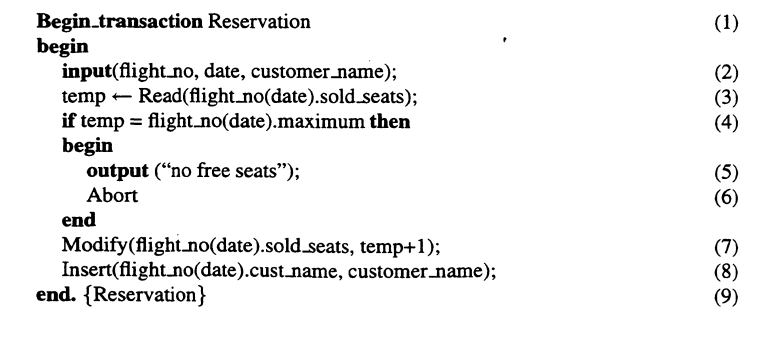
\includegraphics{images}
\end{figure}


Line 1 declares the beginning of the transaction. This is significant, because it notifies the transaction management system that the actions between this point and the "end" command in line 9 are to be executed atomically obeying the ACID properties of transactions. Thus, lines 1 and 9 bracket the transaction. 
Line 2 obtains flight information (flight number, date, and customer's name) from the customer. The seat information about this flight at the specified date is read in line 3 and compared with the maximum number of allowable seats on that flight (line 4). If there are no more seats, then the customer is informed (line 5) and the transaction is aborted (line 6). Aborting a transaction also terminates the transaction (equivalent to an exit). 

If there are available seats (i.e., the transaction does not abort in line 6), the number of sold seats on that particular flight is incremented in line 7. The customer's name is added to the list of customers for that specific flight (line 8), and the transaction successfully completes in line 9. The "Modify" and "Insert" commands constitute the update (also called Write) operations on the database.

The end command in line 9, in addition to syntactically bracketing the transaction definition, also serves the role of an implicit commit command. The importance of commit is twofold. First, the commit command signals that the effects of that transaction should now be reflected in the database, thereby making it visible to other transactions which may access the same data. Second, the point at which a transaction is committed is a "point of no return." The results of the committed transaction are now permanently stored in the database and cannot be undone short of running another transaction to reverse its effects. Thus, commitment implies permanence and visibility of results.


\section*{Types of Transactions}

Transactions have been classified in different ways. One criterion is the duration of transactions other is the type of transaction. Gray classified the transactions as online (short-life) and batch (long-life). Online transactions have a very short execution/response times and relatively affects the small portion of database. This class of transactions probably covers a large majority of current transaction applications. Banking transactions and airline reservation transactions are very good examples of online transactions. In contrast, batch transactions take longer time to execute and have access a large portion of the database. Statistical applications, report generations and image processing are the examples of batch transactions. 


Transactions are also categorized in terms of its read and write actions. If the transactions are restricted so that all the read actions are performed before any write actions, the transaction is called a two-step transaction. Similarly, if the transaction is restricted so that a data item has to be read before it can be updated (written), the transaction is called restricted (or read before-write). If a transaction is both two-step and restricted it is called restricted two-step transaction.

Transactions are also classified in terms of transaction structure.  Flat transactions have a single start point (Begin-transaction) and a single termination point (End-transaction). Most of the transaction management work in databases has concentrated on flat transactions. A nested transaction includes other transactions with their own beginning and tennination points. These transactions that are embedded in another one 
are usually called subtransactions. 


Consider the airline reservation example that was presented. It is quite common for travel agencies to make hotel and rental car arrangements together with airline reservations. It may be preferable to consider all three activities as one unit of execution instead of three separate transactions since they are related to each other. In this case, the reservation transaction would have the following structure:

\begin{figure}[h]
 \centering
 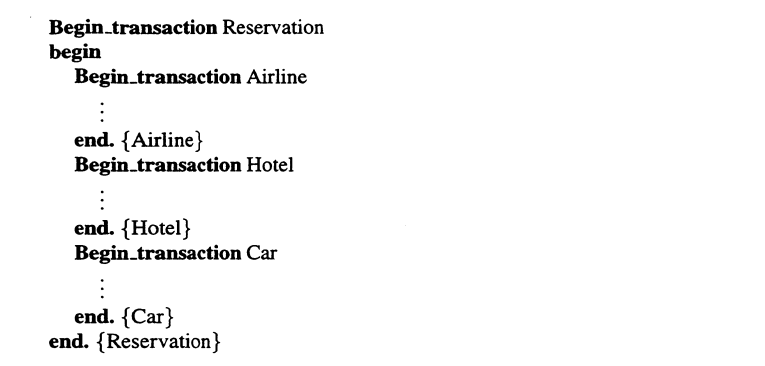
\includegraphics{nested}
\end{figure}

Nested transactions have received considerable interest as a more generalized transaction concept. The level of nesting is generally open, allowing subtransactions themselves to have nested transactions. 


\section*{DBMS States of Transaction}

A database, the transaction can be in one of the following states -

\begin{figure}[h]
 \centering
 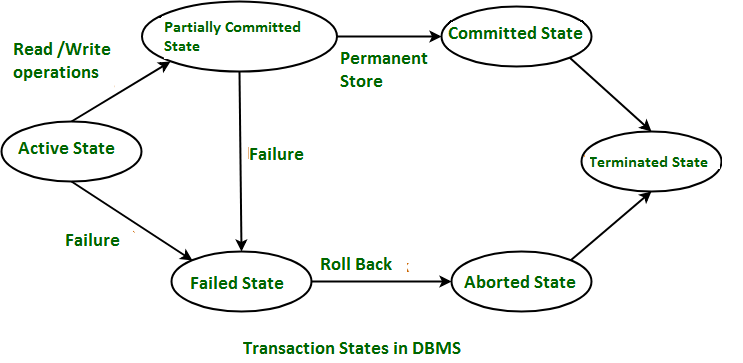
\includegraphics[scale=.7]{states}
\end{figure}

\begin{itemize}

\item Active state

The active state is the first state of every transaction. In this state, the transaction is being executed.
For example: Insertion or deletion or updating a record is done here. But all the records are still not saved to the database.

\item Partially committed

In the partially committed state, a transaction executes its final operation, but the data is still not saved to the database.
In the total mark calculation example, a final display of the total marks step is executed in this state.

\item Committed

A transaction is said to be in a committed state if it executes all its operations successfully. In this state, all the effects are now permanently saved on the database system.

\item Failed state

If any of the checks made by the database recovery system fails, then the transaction is said to be in the failed state.
In the example of total mark calculation, if the database is not able to fire a query to fetch the marks, then the transaction will fail to execute.

\item Aborted

If any of the checks fail and the transaction has reached a failed state then the database recovery system will make sure that the database is in its previous consistent state. If not then it will abort or roll back the transaction to bring the database into a consistent state.
If the transaction fails in the middle of the transaction then before executing the transaction, all the executed transactions are rolled back to its consistent state.

After aborting the transaction, the database recovery module will select one of the two operations:
\begin{itemize}
\item Re-start the transaction
\item Kill the transaction
\end{itemize}

\end{itemize}


\section*{Recovery Management}
The recovery manager is the portion of the database engine that reads and processes the log. It has three functions: to write log records, to roll back a transaction, and to recover the database after a system crash.

In order to be able to roll back a transaction, the recovery manager logs information about the transaction’s activities. In particular, it writes a log record to the log each time a loggable activity occurs. There are four basic kinds of log record: start records, commit records, rollback records, and update records.

Log records are generated by the following loggable activities:
\begin{itemize}


\item A start record is written when a transaction begins.
\item A commit or rollback record is written when a transaction completes.
\item An update record is written when a transaction modifies a value

\end{itemize}

\section*{Concurrency Management}
The concurrency manager is the component of the database engine that is responsible for the correct execution of concurrent transactions. This section examines what it means for execution to be “correct” and studies some algorithms that ensure correctness.

The history of a transaction is the sequence of database actions made by
that transaction, where a database action is the reading or writing of a disk block. When multiple transactions are running concurrently, the database engine will interleave the execution of their threads, periodically interrupting one thread and resuming another. Thus, the actual sequence of operations performed by the concurrency manager will be an unpredictable interleaving of the histories of its transactions. That interleaving is called a \textbf{schedule}.


The purpose of concurrency control is to ensure that only correct schedules get executed. The schedule in which all transactions run serially will not have its operations to be interleaved, that is, the schedule will simply be the back-to-back histories of each transaction. This kind of schedule is called a \textbf{serial schedule}. Concurrency control is predicated on the assumption that a serial schedule has to be correct, since there is no concurrency.

A \textbf{non-serial schedule} is said to be \textbf{serializable} if it produces the same result as some serial schedule. Since serial schedules are correct, it follows that serializable schedules must also be correct.

For an example, consider the following non-serial schedule of the above transactions:\\

W1(b1); W2(b1); W1(b2); W2(b2)\\

Here, W1(b1) means that transaction T1 writes block b1, etc. This schedule
results from running the first half of T1, followed by the first half of T2, the second half of T1, and the second half of T2. This schedule is serializable, because it is equivalent to doing T1 first and then T2. On the other hand, consider the following schedule:\\

W1(b1); W2(b1); W2(b2); W1(b2)\\

This transaction does the first half of T1, all of T2, and then the second half of T1. The result of this schedule is that block b1 contains the values written by T2, but block b2 contains the values written by T1. This result cannot be produced by any serial schedule, and so the schedule is said to be \textbf{non-serializable}.

Recall the ACID property of isolation, which said that each transaction should execute as if it were the only transaction in the system. A non-serializable schedule does not have this property. Therefore, you are forced to admit that non-serializable schedules are incorrect. In other words, a schedule is correct if and only if it is serializable.


\section*{Uses of Transaction Management} 

\begin{itemize}
\item The DBMS is used to schedule the access of data concurrently. It means that the user can access multiple data from the database without being interfered with each other. Transactions are used to manage concurrency.
\item It is used to satisfy ACID properties.
\item It is used to solve Read/Write Conflict.
\item It is used to implement Recoverability, Serializability, and Cascading.
\item Transaction Management is also used for Concurrency Control Protocols and Locking of data.
\end{itemize}

\section*{Disadvantage of using a Transaction} 

\begin{enumerate}

\item It may be difficult to change the information within the transaction database by end-users.
\item We need to always roll back and start from the beginning rather than continue from the previous state.

\end{enumerate}

\section*{Conclusion}


Nowadays many systems become distributed and users can be allowed access to a shared database. The increase in the number of operations on a shared database caused many problems. So we need a control and management tools to ensure a success and security environment for these operations and shared data. Each client program is written as a sequence of transactions. The concurrency manager regulates the execution of these transactions so that they behave consistently. The recovery manager reads and writes records to the log, so that changes made by uncommitted transactions can be undone if necessary. Concurrent transactions can be manage by Concurrency control 
techniques which are providing a serialization among conflicting 
transactions and preventing this conflict.



\end{document}
